\section{Design Document}

\begin{frame}
	\frametitle{Three-tier Architecture}
	\begin{figure}[H]
		\centering
		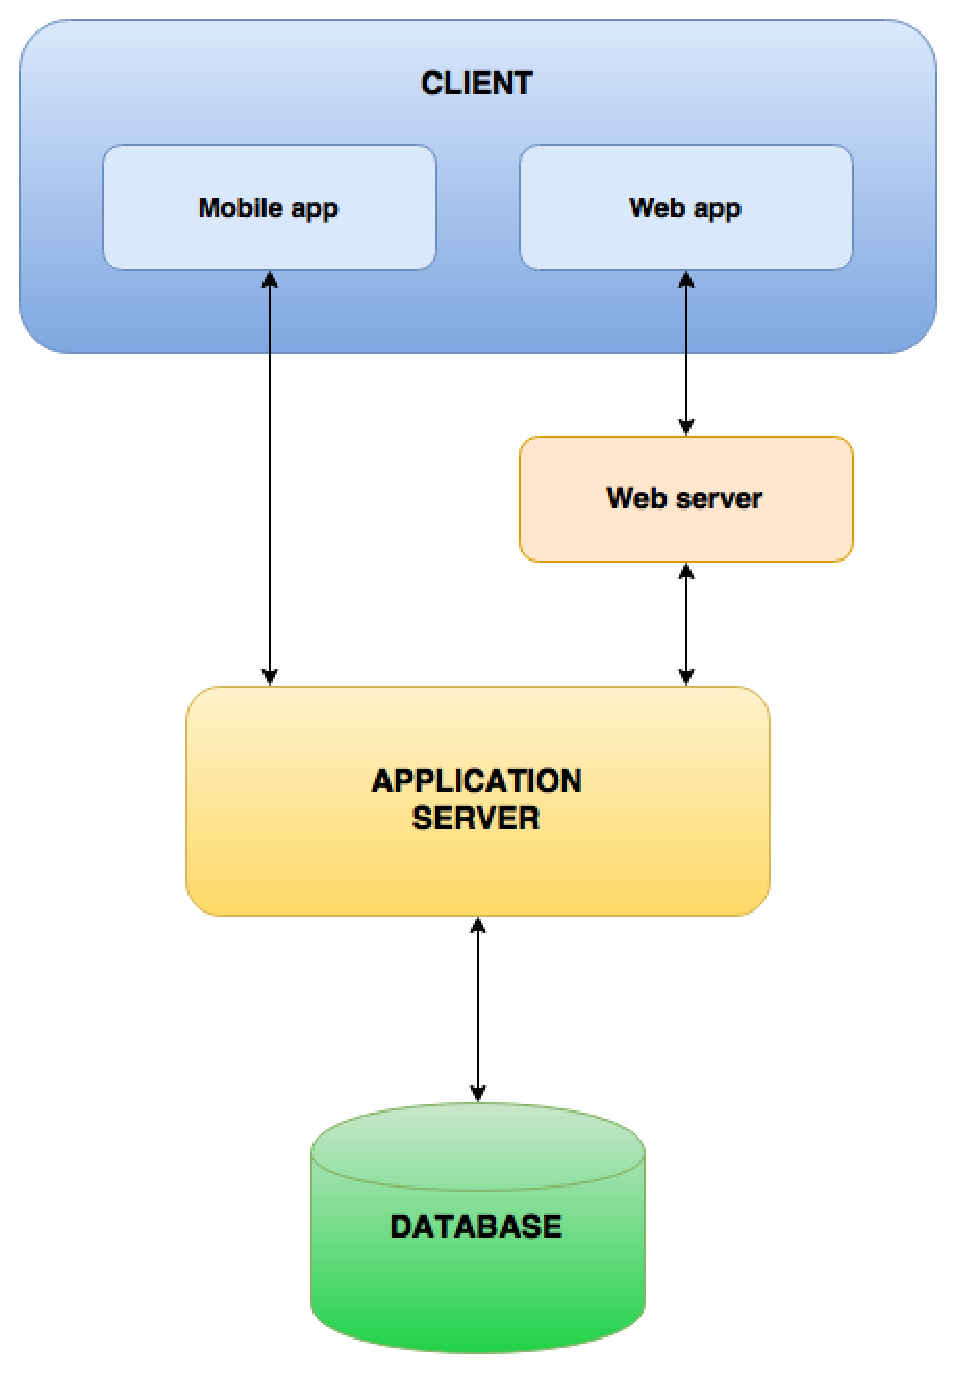
\includegraphics[height=7.3cm,keepaspectratio]{figures/layers.eps}
		\label{fig:layers}
	\end{figure}
\end{frame}

\begin{frame}
	\frametitle{Component View}
	\begin{figure}[H]
		\vspace*{-0.5cm}
		\centering
		\includegraphics[height=12cm,keepaspectratio,angle=270]{figures/component_view.eps}
		\label{fig:component_view}
	\end{figure}
\end{frame}

\begin{frame}
	\frametitle{Deployment View}
	\begin{figure}[H]
		\centering
		\includegraphics[height=7cm,keepaspectratio]{figures/deployment_view.eps}
		\label{fig:deployment_view}
	\end{figure}
\end{frame}

\begin{frame}
	\frametitle{Selection of Available Car}
	\begin{figure}[H]
		\centering
		\includegraphics[height=7cm,keepaspectratio]{figures/selection_available_car.eps}
		\label{fig:selection_available_car}
	\end{figure}
\end{frame}

\begin{frame}
	\frametitle{Reservation of Selected Car}
	\begin{figure}[H]
		\centering
		\includegraphics[height=7.3cm,keepaspectratio]{figures/sequence_reservation.eps}
		\label{fig:sequence_reservation}
	\end{figure}
\end{frame}

\begin{frame}
	\frametitle{UX Diagrams}
	\begin{columns}[c]
		\column{.3\textwidth}
		\begin{figure}[H]
			\centering
			\includegraphics[height=2cm,keepaspectratio]{figures/resv_ux_diagram.eps}
			\label{fig:resv_ux_diagram}
		\end{figure}
		\column{.7\textwidth}
		\begin{figure}[H]
			\centering
			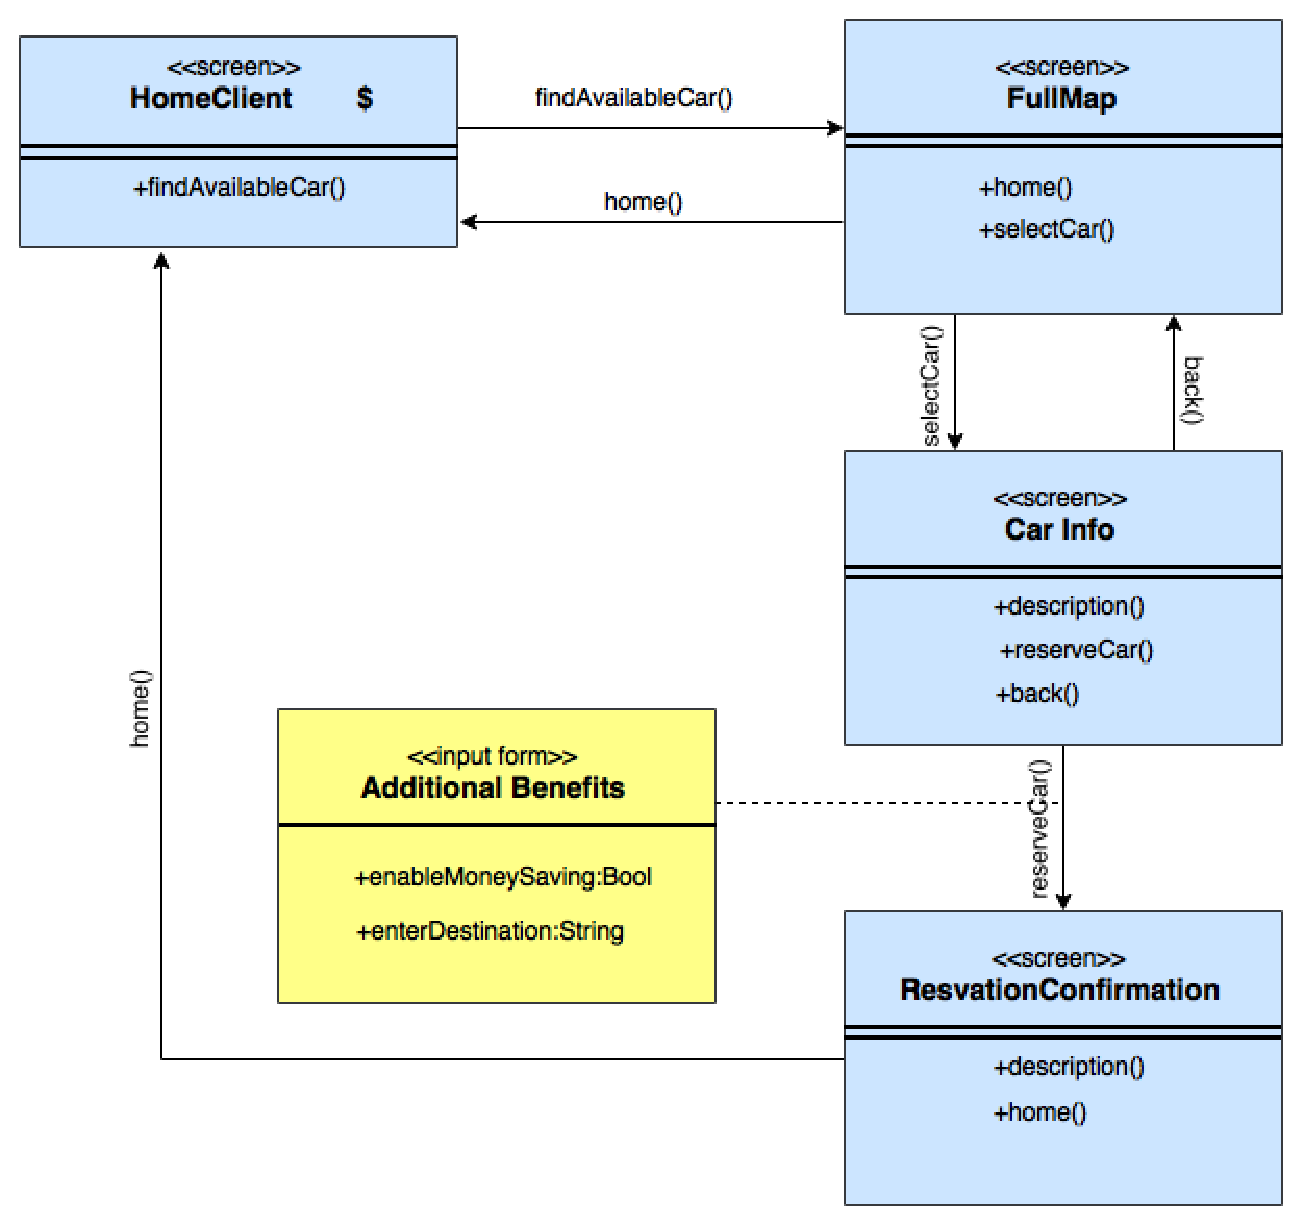
\includegraphics[height=7.3cm,keepaspectratio]{figures/notresv_ux_diagram.eps}
			\label{fig:notresv_ux_diagram}
		\end{figure}
	\end{columns}
\end{frame}